\documentclass{article}

\usepackage{graphicx}
\usepackage{hyperref}
\usepackage{bm}
\usepackage{float}
\restylefloat{table}

\usepackage{listings}
\usepackage{color}
\usepackage{amsmath}

\usepackage[margin=1.25in]{geometry}

\definecolor{dkgreen}{rgb}{0,0.6,0}
\definecolor{gray}{rgb}{0.5,0.5,0.5}
\definecolor{mauve}{rgb}{0.86,0.27,0.22}

\lstset{frame=tb,
  language=python,
  aboveskip=3mm,
  belowskip=3mm,
  showstringspaces=false,
  columns=flexible,
  basicstyle={\small\ttfamily},
  numbers=none,
  numberstyle=\tiny\color{gray},
  keywordstyle=\color{blue},
  commentstyle=\color{dkgreen},
  stringstyle=\color{mauve},
  breaklines=true,
  breakatwhitespace=true,
  tabsize=3
}

%----------------------------------------------------------------------------------------
%	ASSIGNMENT INFORMATION
%----------------------------------------------------------------------------------------

\title{CS5200: Homework \#5} % Title of the assignment

\author{Matthew Whitesides\\ \texttt{mbwxd4@mst.edu}} % Author name and email address

\date{\today} % University, school and/or department name(s) and a date

%----------------------------------------------------------------------------------------

\begin{document}

  \maketitle % Print the title
 
  \begin{enumerate}
    \item \textbf{13.3-2 on p. 322.}
    
    So our goal is to insert and staisfy the cases:

    \begin{enumerate}
      \item All nodes are either red or black.
      \item Leaves are all black.
      \item Red nodes have black children.
      \item Equal number of black nodes in max paths.
      \item All internal nodes have two children – all leaves are NILs and are considered black.
    \end{enumerate}

    Our tree will be built like so {41, 38, 31, 12, 19, 8} (B = Black, R = Red):

    \begin{enumerate}
      \item Insert 41. Result: 41B.
      \item Insert 48. Result: 41B (left)$\rightarrow$ 38R.
      \item Insert 31. Result: 41B (left)$\rightarrow$ 38R (left)$\rightarrow$ 31R.
      \item Recolor 38R to 38B to staisfy case 3. Result: 41B (left)$\rightarrow$ 38B (left)$\rightarrow$ 31R.
      \item Recolor 41B to 41R to staisfy case 4. Result: 41R (left)$\rightarrow$ 38B (left)$\rightarrow$ 31R.
      \item Rotate to the right to balance the tree on 38. Result:\\
      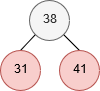
\includegraphics[scale=0.5]{1a.png}
      \item Insert 12 to the left of 31 to result in 12R.
      \item Recolor 31, 41 and 38 to black to keep case 3. Result:\\
      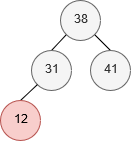
\includegraphics[scale=0.5]{1b.png}
      \item Insert 19R to the right of 12R. 
      \item Rotate left on 12R to put 19R above 12R.
      \item Rotate right on 19R to balance and put 12R and 31 below 19R.
      \item Recolor 19R to black to staisfy caes 4. Result:\\
      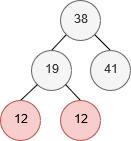
\includegraphics[scale=0.5]{1c.png}
      \item Insert 8R to the left of 12R.
      \item Recolor 12R and 31R to black, and recolor 19B to red to satisfy case 4. Final Result:\\
      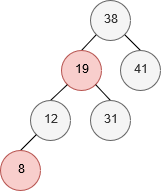
\includegraphics[scale=0.5]{1d.png}

    \end{enumerate}

    \item \textbf{13.4-3 on p. 330.}
    
    Remove {8, 12, 19, 31, 38, 41}:

    \begin{enumerate}
      \item Remove 8:\\
      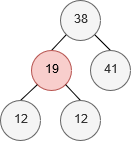
\includegraphics[scale=0.5]{2a.png}
      \item Remove 12.
      \item Recolor 19 to black.\\
      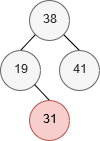
\includegraphics[scale=0.5]{2b.png}
      \item Rotate 19 right to put 31 above 19.
      \item Remove 19.\\
      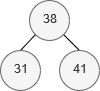
\includegraphics[scale=0.5]{2c.png}
      \item Recolor 31 and 41 to red.
      \item Remove 31.\\
      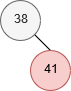
\includegraphics[scale=0.5]{2d.png}
      \item Remove 41.\\
      
\includegraphics[scale=0.5]{2e.png}
      \item Finally remove 38.
    \end{enumerate}

    \item \textbf{15.2-2 on p. 378. Implement your algorithm.}
    \item \textbf{15.4-1 on p. 396.}
    \item \textbf{15.4-5 on p. 397. Just describe the algorithm.}
    \item \textbf{16.1-3 on p. 422.}
    \item \textbf{16.2-5 on p. 428. Just describe the algorithm.}
    \item \textbf{16.3-3 on p. 436.}
    \item \textbf{17.4-3 on p. 471.}
    \item \textbf{18.2-1 on p. 497.}
    \item \textbf{18.3-1 on p. 350.}
    \item \textbf{19.2-1 on p. 518.}
    \item \textbf{19.4-1 on p. 526.}
    \item \textbf{21.3-2 on p. 572. Implement your algorithm.}
  \end{enumerate}

\end{document}
